\subsubsection{标注工具}
\textbf{labelImg介绍:}为了方便使用自己的数据集进行深度学习训练,需要对图片进行标注。本文使用labelImg,这是一款被广泛使用的图片标注工具。
\begin{uscfigure}
	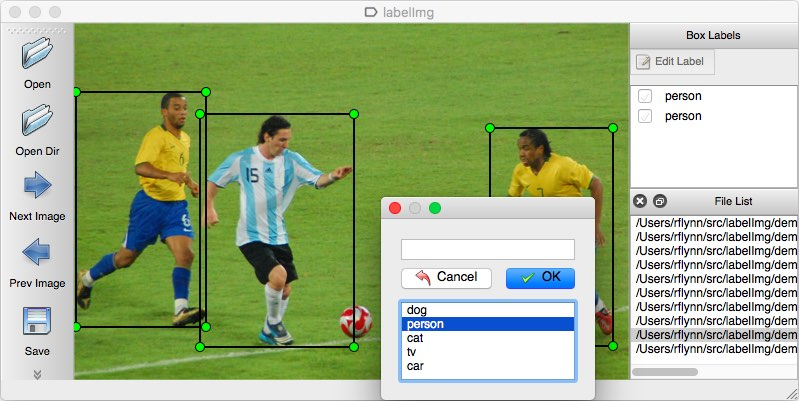
\includegraphics[width=\textwidth]{./Pictures/labelimg.jpg}	
	\caption{labelImg界面}
\end{uscfigure}
\subsubsection{数据集}
\textbf{VOC数据集介绍:}PASCAL VOC为图像分类、目标检测等任务的需要提供了标准的数据库。系统的目标检测任务只需要使用JPEGImage、Annotations、ImageSets三个文件夹。将受损的瓦片图片放入JPEGImage文件夹,将对应的保存为.xml文件的标注信息放入Annotations文件夹。

其目录结构为:

- JPEGImages:将受损瓦片的图片放入此文件夹,图片大小为224*224像素;

- Annotations:将JPEGImages文件夹中对应图片的标注信息放入此文件夹,其文件格式为xml;

- ImageSet:此处将训练、测试、验证等图片的信息放到此处,方便程序的读写。


\subsubsection{Pytorch介绍}
PyTorch是深度学习框架,因为非常易于使用,所以被非常多的研究人员所喜爱。PyTorch支持动态计算图非常有吸引力。
\subsubsection{OpenCV介绍}
OpenCV是一个开源的计算机视觉库,他实现了图像处理和计算机视觉方面的非常多的通用算法。底层由C/C++语言写成,所以运行速度快,跨平台支持挺好。
\subsubsection{将图片切割成300px大小}
\begin{lstlisting}[caption={图像切割}]
img = img.resize(self.img_size, self.img_size)
\end{lstlisting}

输入的图片其大小为300*300大小的像素,利用OpenCV函数库提供的resize函数对图片进行大小的设定。